\documentclass[10pt, twocolumn]{report}

% гипер ссылки
\usepackage{cmap} % чтобы был поиск по pdf

\usepackage[utf8]{inputenc}
\usepackage[english, russian]{babel}
\usepackage[T2A]{fontenc}
\usepackage[unicode]{hyperref}

\usepackage{xcolor}
\usepackage{hyperref}
\usepackage{svg}
\usepackage{pdfpages}


% русские буквы в формулах
\usepackage{mathtext}
\usepackage{amsmath,amsfonts,amssymb,amsthm,mathtools}
\usepackage{longtable}
\usepackage{multirow}


\usepackage[left=15mm, right=15mm, top=15mm, bottom=15mm, landscape, a3paper]{geometry}
\tolerance=314

%%%%%%%%%%%%%%%%%%%%%%%%%%%%%%%%%%%%%%%%%%%%%%%%
%%% добавляем точки в Оглавление

\renewcommand{\thechapter}{\arabic{chapter}.}
\renewcommand{\thesection}{\arabic{chapter}.\arabic{section}.}
\renewcommand{\thesubsection}{\arabic{chapter}.\arabic{section}.\arabic{subsection}.}


\newenvironment{itemize*}%
{\begin{itemize}%
	\setlength{\itemsep}{1pt}%
	\setlength{\parskip}{1pt}}%
{\end{itemize}}

\newenvironment{enumerate*}%
{\begin{enumerate}%
	\setlength{\itemsep}{1pt}%
	\setlength{\parskip}{1pt}}%
{\end{enumerate}}


% отступ при наборе формул в блоке multline
\multlinegap=2cm
% будем считать что переполнения не было, если строка вышла за границу не более чем 0.01pt
\hfuzz=0.01pt
% разрешаю увеличить расстояние между словами не больше чем на 14pt, что бы не было переполнения
\emergencystretch=14pt
% изменение межстрочного интервала
\def\heightline{1.1}
\linespread{\heightline} % 1.3 - это полуторный

\usepackage{hyperref}
%\usepackage[usenames,dvipsnames,svgnames,table,rgb]{xcolor}
\hypersetup{				% Гиперссылки
	unicode=true,           % русские буквы в раздела PDF
	pdftitle={Заголовок},   % Заголовок
	pdfauthor={Автор},      % Автор
	pdfsubject={Тема},      % Тема
	pdfcreator={Создатель}, % Создатель
	pdfproducer={Производитель}, % Производитель
	pdfkeywords={keyword1} {key2} {key3}, % Ключевые слова
	colorlinks=true,       	% false: ссылки в рамках; true: цветные ссылки
	linkcolor=red,          % внутренние ссылки
	citecolor=black,        % на библиографию
	filecolor=magenta,      % на файлы
	urlcolor=cyan           % на URL
}

\title{\textbf{\Huge{Проект одноэтажного загородного дома}}}
\author{ Морозов Андрей }
\date{Нижний Новгород, 2015-2017}


\begin{document}
\maketitle

\tableofcontents

\part{О проекте}

\chapter{Проектирование}

Встал вопрос в чем проектировать и как. Есть огромное количество иструментов и еще большее количество, о которых я не ничего не знаю. 

Проектирование(черчение) и подготовка проектной документации велась во LibreCAD\footnote{LibreCAD - \href{http://librecad.org}{http://librecad.org}}.

\chapter{Зарубежный опыт}

\newcommand{\kwpm}{$\cfrac{\text{кВт·ч}}{\text{м}^2}\ $}

\section{Пассивные дома}
Пассивный дом, энергосберегающий дом, или экодом (нем. Passivhaus, англ. passive house) -- сооружение, основной особенностью которого является отсутствие необходимости отопления или малое энергопотребление - в среднем около 10\% от удельной энергии на единицу объёма, потребляемой большинством современных зданий. В большинстве развитых стран существуют собственные требования к стандарту пассивного дома.

Растут цены на электричество и тепло. Остро стоит вопрос эксплуатационных затрат на жилье. Показателем энергоэффективности объекта служат потери тепловой энергии с квадратного метра \kwpm в год или в отопительный период. В среднем составляет 100—120 \kwpm. Энергосберегающим считается здание, где этот показатель ниже 40 \kwpm.Для европейских стран этот показатель ещё ниже — порядка 10 \kwpm.

Достигается снижение потребления энергии в первую очередь за счет уменьшения теплопотерь здания.

В Европе существует следующая классификация зданий в зависимости от их уровня энергопотребления:
\begin{itemize}
	\item "Старое здание" (здания построенные до 1970-х годов) — они требуют для своего отопления около трехсот киловатт-часов на квадратный метр в год: 300 \kwpm год.
	\item "Новое здание" (которые строились с 1970-х до 2000 года) — не более 150 \kwpm год.
	\item "Дом низкого потребления энергии» (с 2002 года в Европе не разрешено строительство домов более низкого стандарта) — не более 60 \kwpm год.
	\item "Пассивный дом" — не более 15 \kwpm год.
	\item "Дом нулевой энергии" (здание, архитектурно имеющее тот же стандарт, что и пассивный дом, но инженерно оснащенное таким образом, чтобы потреблять исключительно только ту энергию, которую само и вырабатывает) — 0 \kwpm год.
	\item "Дом плюс энергии" или "активный дом" (здание, которое с помощью установленного на нём инженерного оборудования: солнечных батарей, коллекторов, тепловых насосов, рекуператоров, грунтовых теплообменников и т. п. вырабатывало бы больше энергии, чем само потребляло).
	
\end{itemize}

\section{Энергосберегающие дома}


\section{Экономическая выгода}
В России энергопотребление в домах составляет 400—600 \kwpm в год.

\section{Инструмент и спецодежда}

Пневмоинструмент наше все, одежда защищает от травм.

Инструмент:

\begin{itemize}
	\item Измерительная рулетка
	\item Электролобзик
	\item Молотки (600гр, 700гр, 800гр, 900гр)
	\item Гвоздодер
	\item Шуроповерт
	\item Уровень, угольник
	\item Струбцины
	\item Циркулярная электропила
	\item Радиально отрезной станок
	\item Дрель ударная
	\item Пневмо шлифовальная машина
%	\item ...
\end{itemize}

\part{Земельный участок}
\chapter{Расположения объектов на земельном участке}
Согласно СП 53.13330.2011, жилое строение или жилой дом должны отстоять от красной линии улиц не менее чем на 5 м, от красной линии проездов — не менее чем на 3 м. При этом между домами, расположенными на противоположных сторонах проезда, должны быть учтены противопожарные расстояния. Расстояния от хозяйственных построек до красных линий улиц и проездов должны быть не менее 5 м. По согласованию с правлением садоводческого, дачного объединения навес или гараж для автомобиля может размещаться на участке, непосредственно примыкая к ограде со стороны улицы или проезда.

Минимальные расстояния до границы соседнего участка по санитарно-бытовым условиям должны быть от:
\begin{itemize*}
	\item жилого строения (или дома) — 3 м;
	\item постройки для содержания мелкого скота и птицы — 4 м;
	\item других построек — 1 м;
	\item стволов высокорослых деревьев — 4 м, среднерослых — 2 м;
	\item кустарника — 1 м.
\end{itemize*}

Расстояние между жилым строением (или домом), хозяйственными постройками и границей соседнего участка измеряется от цоколя или от стены дома, постройки (при
отсутствии цоколя), если элементы дома и постройки (эркер, крыльцо, навес, свес крыши и др.) выступают не более чем на 50 см от плоскости стены. Если элементы
выступают более чем на 50 см, расстояние измеряется от выступающих частей или от проекции их на землю (консольный навес крыши, элементы второго этажа, расположенные на столбах и др.).

При возведении на садовом, дачном участке хозяйственных построек, располагаемых на расстоянии 1 м от границы соседнего садового, дачного участка, скат
крыши следует ориентировать таким образом, чтобы сток дождевой воды не попал на соседний участок.


Минимальные расстояния между постройками по санитарно-бытовым условиям должны быть, м:
\begin{itemize*}
	\item от жилого строения или жилого дома до душа, бани (сауны), уборной — 8;
	\item от колодца до уборной и компостного устройства — 8.
\end{itemize*}

Указанные расстояния должны соблюдаться между постройками, расположенными на смежных участках.

В случае примыкания хозяйственных построек к жилому строению или жилому дому расстояние до границы с соседним участком измеряется отдельно от каждого объекта блокировки, например:

\begin{itemize*}
	\item дом-гараж (от дома не менее 3 м, от гаража не менее 1 м);
	\item дом-постройка для скота и птицы (от дома не менее 3 м, от постройки для скота и птицы не менее 4 м).
\end{itemize*}

Гаражи для автомобилей могут быть отдельно стоящими, встроенными или пристроенными к садовому, дачному дому и хозяйственным постройкам.

\chapter{План земельного участка}
Вот земля, нужно разместить все постройки в соответствие с гостом.	

\begin{figure}[h]
	\centering
	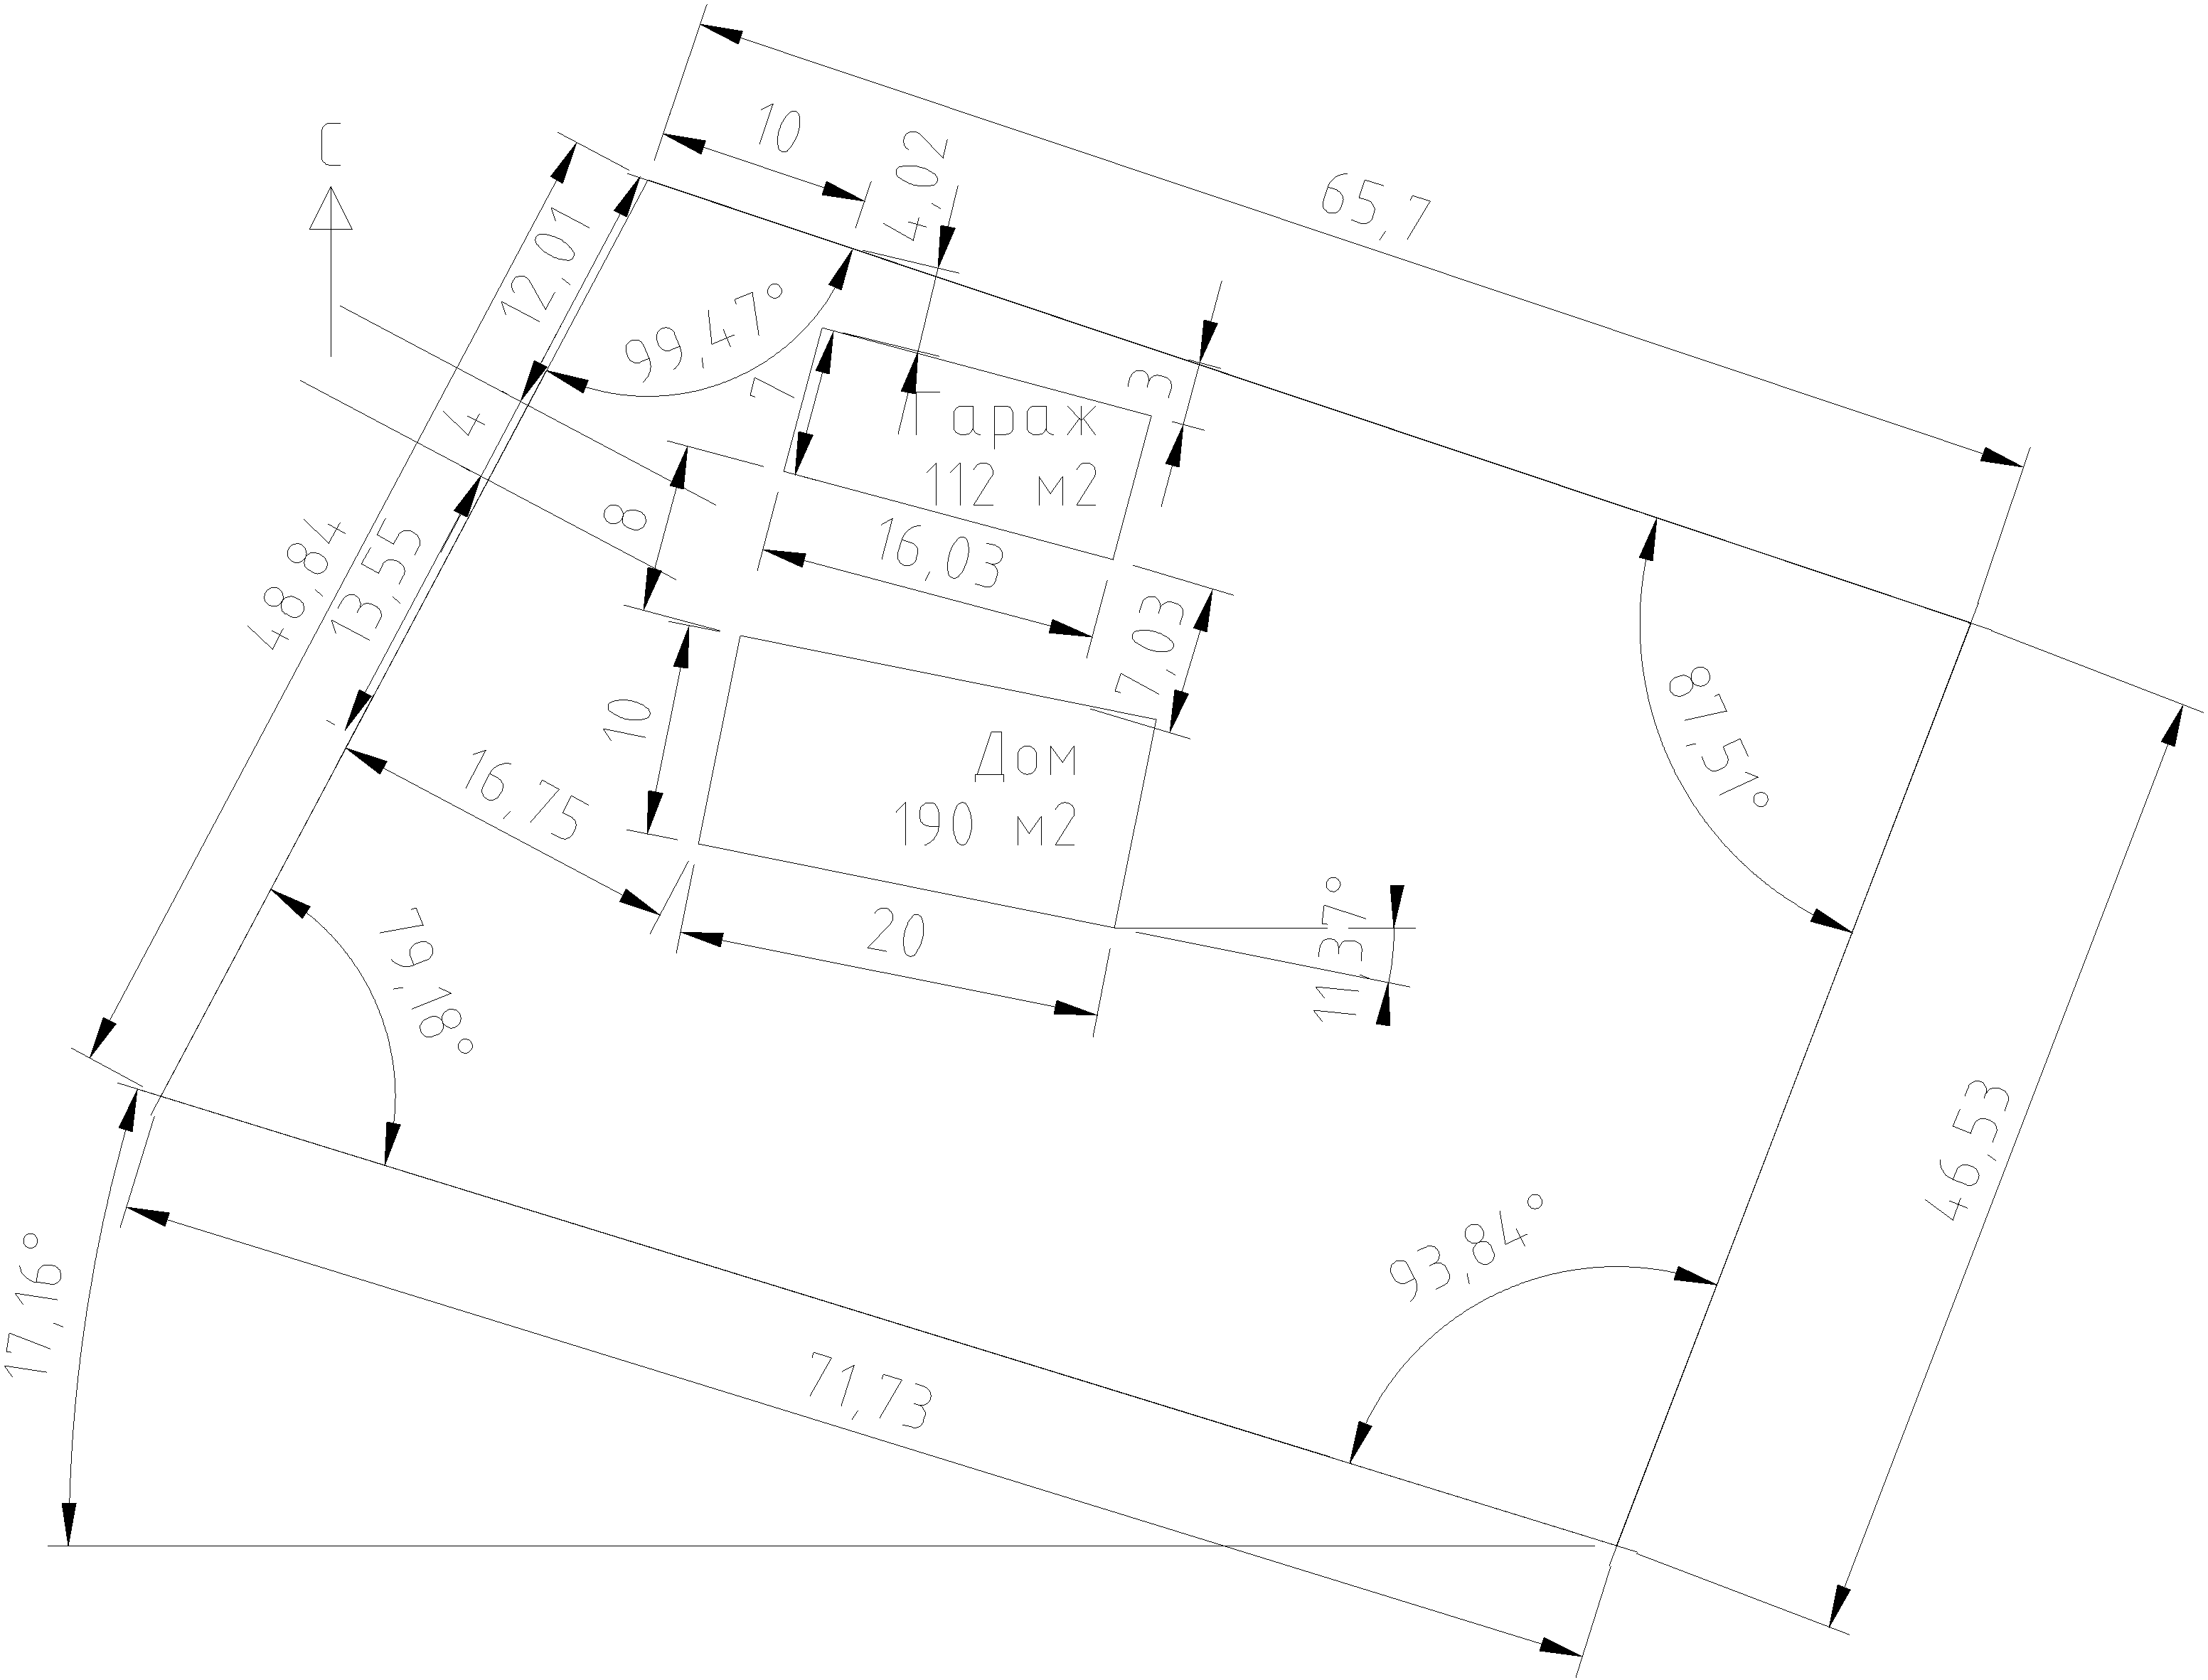
\includegraphics[height=0.85\textheight]{img/area.png}
	\caption{Земельный участок}
	\label{fig:area}
\end{figure}


\part{Архитектура}
\chapter{План дома}
Что нам стоит дом построить, нарисуем будем жить.

\begin{figure}[h]
	\centering
	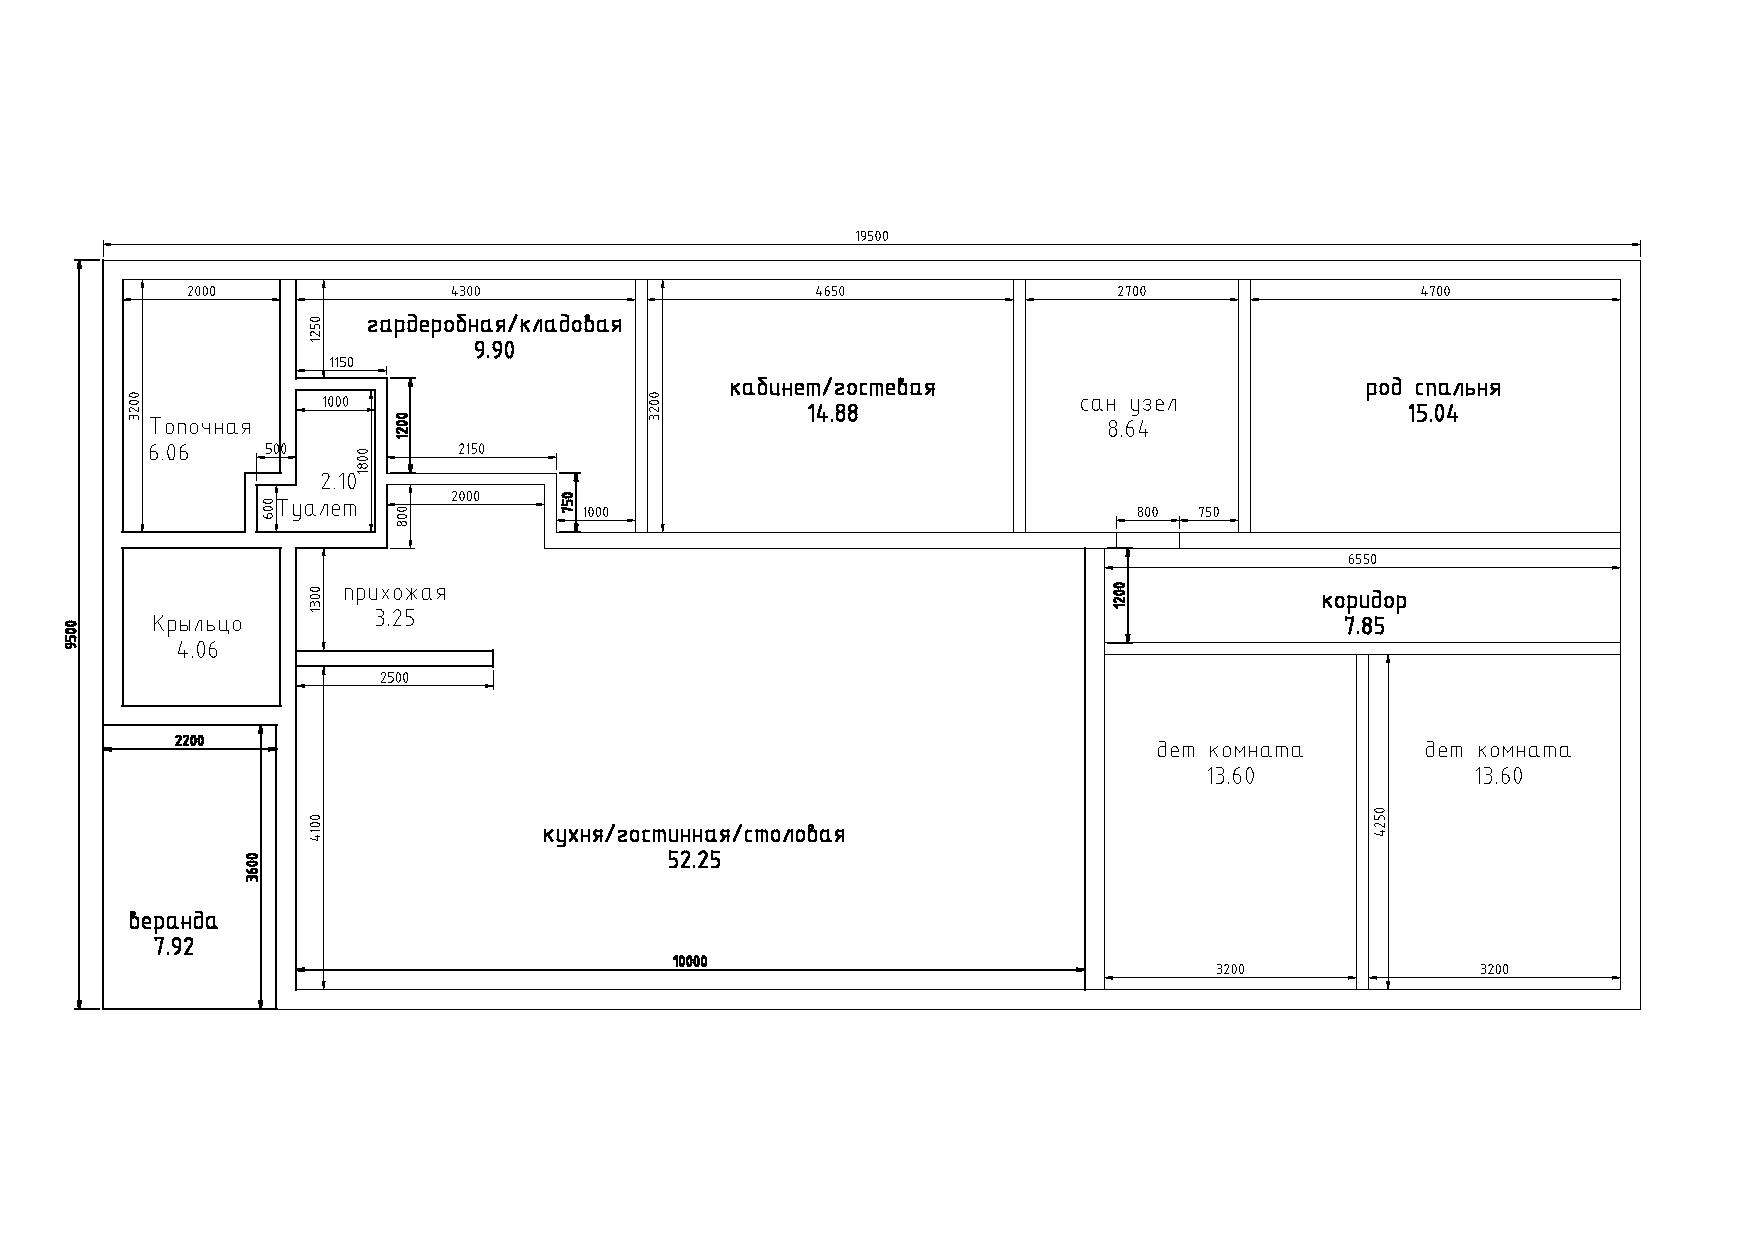
\includegraphics[width=1.0\textwidth]{img/plan.pdf}
	\caption{План дома}
	\label{fig:plan}
\end{figure}

\chapter{Фундамент}

Существует несколько типов фундаментов со своими плюсами и минусами.

\chapter{Первый этаж}

Пирог стены:
Пароизоляция Ютафол Н 110.

Окна монтируются в ЭППС, для предотвращения конденсата на окнах и их промерзания.

кирпичная кладка - М150
раствор - М75-М100
первый ряд - гидроизоляционный раствор 1:1 (1:2) (можно с добавлением жидкого стекла) + евроруберойд на синтетической основе(стеклохолст) с толщиной не менее 3 мм

наплавляемая гидроизоляция

Б20 бетон

\chapter{Крыша}

\chapter{Окна}

Определим размер окон из условий расположений каркаса дома.

Для спален, кабинета, коридора и кухни поместим окно между двумя стойками каркаса -- размер \textbf{проема} под окна $1100 \times 1500$. Для зала, большое окно будет иметь размеры $1725 \times 1500$. 

\chapter{Веранда}

\part{Коммуникации}

\chapter{Разное}

Контроллер Esbe серии CRB100
http://pdf.heiz.ru/esbe-crb100-tech.pdf

\chapter{Отопление}
У нас есть до 12 квт на отопление в ночное время, днем до 4.5 квт.

Радиаторы под окна + теплые полы.

Размеры стальных радиаторов:
H - высота (300, 400, 450, 500, 600, 900)
L - длинна (400, 500, 600, 700, 800, 900, 1000, 1100, 1200, 1400, 1600, 1800, 2000, 2300, 2600, 3000)

под размеры окон(шириной): 1000, 1200, 2000

высотой: высота потолков - 900мм от пола и 400мм от потолка $=>$ (3.0 ... 3.5) - 0.9 - 0.4 = 1.7 ... 2.2 м

\chapter{Водоснобжение}
Расчет систем водоснабжения производится исходя из следующих норм среднесуточного водопотребления на хозяйственно-питьевые нужды:

\begin{itemize*}
	\item при водопользовании из водоразборных колонок, скважин, шахтных колодцев -- 30-50 л/сут на 1 жителя;
	\item при обеспечении внутренним водопроводом и канализацией (без ванн) -- 125-160 л/сут на 1 жителя.
	\item Для полива посадок на приусадебных участках: овощных культур -- 3-15 л/м2 в сутки; плодовых деревьев -- 10-15 л/м2 в сутки.
\end{itemize*}

Для полива предполагаетсяя использовать черный бак на 3.5 куба, который заполняется водой ночью, днем нагревается и вечером используется для полива огорода. А ночью опять заливается.

\chapter{Электричество}
У нас есть 15квт, нужно распорядится ими по умному, незабывая закон Ома $$ I = \cfrac{U}{R} $$

\section{Подключение электричества}

\subsection{Технические условия}

Категория надежности - 3 категории - 15 кВт.
Ответвление от точки епррисоединения к вводу в здание должно быть выполнено самонесущим кабелем изолированным проводом сечением не менее 16 $\text{мм}^2$. Крепление к стене здания выполнить в месте не подверженном сходу снега.

\textbf{Требования к устройствам обеспечивающим контроль велечины максимальной мощности} -- установить вводной аппарат автоматической защиты (защиты могут быть комбинированными). Установку по току выбрать в зависимости от заявленной мощности и напряжения. Аппарат должен имень функцию ручного отключения. 

\textbf{Требования к приборам релейной защиты и автоматики} -- выполнить установку аппаратом защиты от грозовых коммутационных напряжений, аппаратов защиты от повышенного напряжения возникающего в 3-х фазных сетях при обрывы PEN проводника. Выполнить заземление и зануление электроприемников. Аппараты релейной защиты могут быть расположены как в ШУ, так и в ВРУ.

\textbf{Требования к приборам учеты электрической энергии} -- Щит учета устанавливается на границе балансовой принадлежности, либо в иных местах, наиболее приближенных к границе балансовой принадлежности(вне территории жилого помещения, на вводе в дом), с применением выносных пунктов учета, с установкой многофункционального электронного прибора учета электрической энергии, класса точности 2,0 и выше. Щит учета должен обеспечивать съем показаний счетчика без его открывания или с открытием без помощи ключа. Металлический корпус ЩУ необходимо заземлить, $\sum{R_{\text{З}}} = \frac{R_{\text{щу}} \cdot R_{\text{вру}}}{R_{\text{щу}} + R_{\text{вру}}} \le 10 \text{ Ом}$. Щит учета может быть совмещен с ВРУ.

\subsection{Разновидности систем искусственного заземления}

Классификация типов систем заземления приводится в качестве основной из характеристик питающей электрической сети. ГОСТ Р 50571.2-94 «Электроустановки зданий. Часть 3. Основные характеристики» регламентирует следующие системы заземления: TN-C, TN-S, TN-C-S, TT, IT.

Для электроустановок напряжением до 1 кВ приняты следующие обозначения:

\begin{itemize}
\item система TN — система, в которой нейтраль источника питания глухо заземлена, а открытые проводящие части электроустановки присоединены к глухозаземлённой нейтрали источника посредством нулевых защитных проводников;
\item система TN-С — система TN, в которой нулевой защитный и нулевой рабочий проводники совмещены в одном проводнике на всём её протяжении;
\item система TN-S — система TN, в которой нулевой защитный и нулевой рабочий проводники разделены на всём её протяжении;
\item система TN-C-S — система TN, в которой функции нулевого защитного и нулевого рабочего проводников совмещены в одном проводнике в какой-то её части, начиная от источника питания;
\item система IT — система, в которой нейтраль источника питания изолирована от земли или заземлена через приборы или устройства, имеющие большое сопротивление, а открытые проводящие части электроустановки заземлены;
\item система ТТ — система, в которой нейтраль источника питания глухо заземлена, а открытые проводящие части электроустановки заземлены при помощи заземляющего устройства, электрически независимого от глухозаземлённой нейтрали источника.
\end{itemize}

ТИП TN-C
\includegraphics[scale=1]{img/tn-c.pdf}

ТИП TN-S
\includegraphics[scale=1]{img/tn-s.pdf} 

ТИП TN-C-C
\includegraphics[scale=1]{img/tn-c-s.pdf} 

\subsubsection{Система TN-C-S}
В системе TN-C-S трансформаторная подстанция имеет непосредственную связь токопроводящих частей с землёй и наглухо заземлённую нейтраль. Для обеспечения связи на участке трансформаторная подстанция — ввод в здание применяется совмещённый нулевой рабочий (N) и защитный проводник (PE), принимающий обозначение PEN. При вводе в здание он (PEN) разделяется на отдельный нулевой (N) и защитный проводник (PE).

\begin{itemize}
\item Также можно наблюдать систему TN-C-S, где разделение нулей происходит в середине линии, однако, в случае обрыва нулевого провода до точки разделения, корпуса окажутся под линейным напряжением, что будет представлять угрозу для жизни при касании.
\item Достоинства: более простое устройство молниезащиты (невозможно появление пика напряжения между PE и N), возможность защиты от КЗ фазы на корпус прибора с помощью обыкновенных «автоматов».
\item Недостатки: крайне слабая защищённость от «отгорания нуля», то есть разрушения PEN по пути от КТП к точке разделения. В этом случае на шине PE со стороны потребителя появляется фазное напряжение, которое не может быть отключено никакой автоматикой (PE не подлежит отключению). Если внутри здания защитой от этого служит система уравнивания потенциалов (СУП) (под напряжением оказывается всё металлическое, и нет риска поражения током при прикосновении к 2 разным предметам), то на открытом воздухе никакой защиты от этого не существует вовсе.
\end{itemize}

В соответствии с ПУЭ является основной и рекомендуемой системой, но при этом ПУЭ требуют соблюдения ряда мер по недопущению разрушения PEN — механическую защиту PEN, а также повторных заземлений PEN воздушной линии по столбам через какое-то расстояние (не более 200 метров для районов с числом грозовых часов в году до 40, 100 метров для районов с числом грозовых часов в году более 40).

В случае, когда эти меры соблюсти невозможно, ПУЭ рекомендуют TT. Также ТТ рекомендуется для всех установок под открытым небом (сараи, веранды и т. д.)

В городских зданиях шиной PEN обычно является толстая металлическая рама, вертикально идущая через всё здание. Её практически невозможно разрушить, потому в городских зданиях применяется TN-C-S.

В сельской же местности в России на практике существует огромное количество воздушных линий без механической защиты PEN и повторных заземлений. Потому в сельской местности более популярна система TT.

В позднесоветской городской застройке как правило применялась TN-C-S с точкой деления на основе электрощита (PEN) рядом со счетчиком, при этом PE проводилась только для электроплиты.

В современной российской застройке применяется и «пятипроводка» с точкой деления в подвале, в стояках проходят уже независимые N и PE. 

\subsection{Закупка комплектующих и сборка щитка}

Комплектующие:
\begin{itemize}
	\item 32А трехфазный.
	\item Щит учетно-распределительный навесной ЩУРн-3/12 IP54 (mb54-3) EKF или Щит навесной TDM ЩУ 3/1-0-12 12 модулей и место под трехфазный счетчик с металлической дверцей с замком и окном IP66 
	\item Автоматический выключатель Schneider Electric Acti9 iK60N 3P 32А характеристика C
	\item УЗО Schneider Electric Acti9 iID 4P 40А 300мА класс AC
	\item Ограничитель импульсных перенапряжений IEK ОПС1-C 3P 20кА класс C
\end{itemize}

Номинал УЗО должен быть выше номинала автомата в 1.5 раза.


\section{Провода и автоматы}
провода и автоматы:

\begin{tabular}{|l|c|c|c|}
\hline
\multirow{2}{*}\textbf{Назначение} & \textbf{Сечение} & \textbf{Номинал} & \textbf{Максимальная} \\
& \textbf{провода} & \textbf{автомата} & \textbf{мощность в квт} \\
\hline
\textbf{Освещение и подсветка} & $1.5 \text{мм}^2$ & \textbf{10А} & \textbf{2.30 квт} \\
\textbf{Розетки, кондиционеры, балконы} & $2.5 \text{мм}^2$ & \textbf{16А} & \textbf{3.68 квт} \\
\textbf{Электрический духовой шкаф} & $4.0 \text{мм}^2$ & \textbf{20А} & \textbf{4.60 квт} \\
\textbf{Варочная панель, водонагреватель} & $6.0 \text{мм}^2$ & \textbf{25А} & \textbf{5.75 квт} \\
\hline
\end{tabular}

Предпочитаемые автоматы.
\begin{enumerate}
\item Schneider Electric IC60N, IK60N - Франция, Тайланд (исключить Easy 9 - Индия)
\item ABB S201 - Германия
\item ---
\item IEK BA47-29 - Россия/Китай
\item EKF BA47-63 - Россия/Китай
\item ---
\item ELVERT - Россия/Китай
\item KEAZ - Россия/Китай
\item TDM  - Россия/Китай
\end{enumerate}


\begin{enumerate}
\item Автоматический выключатель Schneider Electric Acti9 iK60N 1P 6А характеристика C
\item Автоматический выключатель Schneider Electric Acti9 iK60N 1P 10А характеристика C
\item Автоматический выключатель Schneider Electric Acti9 iK60N 1P 16А характеристика C
\item Автоматический выключатель Schneider Electric Acti9 iK60N 1P 20А характеристика C
\item Автоматический выключатель Schneider Electric Acti9 iK60N 1P 25А характеристика C
\item Дифференциальный автоматический выключатель Schneider Electric Acti9 iDif K 2Р 10А 30мА класс AC
\item Дифференциальный автоматический выключатель Schneider Electric Acti9 iDif K 2P 16А 30мА класс AC
\item Дифференциальный автоматический выключатель Schneider Electric Acti9 iDif K 2P 20А 30мА класс AC
\item Дифференциальный автоматический выключатель Schneider Electric Acti9 iDif K 2P 25А 30мА класс AC
\item 
\item УЗО Schneider Electric Acti9 iID 2P 25А 30мА класс AC
\item УЗО Schneider Electric Acti9 iID 2P 40А 30мА класс AC
\item УЗО Schneider Electric Acti9 iID 4P 40А 300мА класс AC
\item 
\end{enumerate}

\chapter{Водопроврод}
Будем использовать трубы рихау и все тут.

\chapter{Вентиляция}
Стандарт говорит, что воздух нам нужен.

Вопрос в том что непонятно сколько. Возможно достаточно проветривать помещение раз в день - перед сном.

С каждым годом стоимость отопления увеличивается и в погоне за экономией мы стараемся сберечь тепло, которе у нас есть в доме, применяя порой очевидные приемы, которые помогут нам в этом, однако забывая о последствиях. В старых СНиПах 80-х годов было указано, что окна в домах \textbf{должны} обеспечить определенный приток воздуха в помещение. Было дано вполне определенное число по стандарту, сколько иммено воздуха окно должно пропускать. В свою очередь, поступление холодного воздуха в дом сильно его охлаждает. Такие старые окна окна меняют на современные пластиковые которые сохраняют тепло и не пропускают холодный воздух снаружи внутрь дома. В результате обновление свежего воздуха в доме просто останавливается. 

Про проведенным экспериментам из статьи \cite{co2}, следует что:
В помещение площадью 15 $\text{м}^{2}$ (кубатура: 37.5 $\text{м}^3$ - потолок 2.5м), два человека в комнате. 
Проветривание одним окном. Концентрация углекислого газа в этом случае упала с 1765 ppm до 799 ppm (из «красной» зоны в «зелёную») за 12 минут и 17 секунд.
Один человек в комнате и проветривание двумя окнами. 
Проветривание ранним ноябрьским утром дало уменьшение концентрации углекислого газа с 2070 ppm до 763 ppm за 5 минут и 37 секунд.
Следующий эксперимент, прогрев воздуха кондеционером.
В комнате во время замеров было 2 человека. Получилось, что при работающем кондиционере (в режиме "+25, Солнышко") концентрация углекислого газа выросла с комфортных 591 ppm до «красной зоны» в 1200 ppm за 28 минут и 47 секунд.

Кстати, при выключенном кондиционере ситуация похожая. В этой же комнате уровень CO2 растёт с 0,06\% до 0,12\% тоже примерно за полчаса (если в комнате 2 человека). А часа за 2 он доходит до критической отметки 0,3\%, и, по возможности, весьма желательно уже проветривать (хоть на улице и зима :) ).

Как видно из эксперимента при наличии 2 человек в большой 15 метровой комнате необходиом проветривать помещение каждые 2 часа по 15 мин, а лучше чаще.

Если проветривать реже то это очень скажется на самочувствие.  

\section{Нормы воздухообмена}

При рассчетах обычно опираются на 30 $\text{м}^3$ на человека в час или 1 объем помещения в час.

Как такие параметры достичь. Вариантов несколько:

\begin{itemize*}
	\item Естественная вентиляция. В простейшем случае вытяжные каналы (трубы) из санузлов и кухни на крышу и приток свежего воздуха через форточки. Дешево и сердито.
	\item  Вытяжка принудительная, приток естественный. То есть в вытяжных каналах ставятся вентиляторы. Работают они либо постоянно, либо по датчикам (например, влажности или присутствия в ванной или CO2 в жилых помещениях). Приток опять же либо через форточки, либо через приточные клапаны.
	\item Вытяжка естественная, притокт принудительный.
	То есть в спальнях ставятся системы типа Бризер Tion O2(это приточная вентиляция для квартиры или офиса), а вытяжка через вытяжные канали в сан узлах.
	\item Полноценная приточно-вытяжная система с подачей воздуха в жилые помещения и его забором из нежилых. Переток воздуха в доме осуществляется через щели под дверьми или же через переточные решетки. Часто используется с рекуператором.
\end{itemize*}. 


\part{Расчеты}

\chapter{Нагрузка на кровлю}

Деревня недалеко от Нижнего Новгорода.

\section{Снеговая нагрузка}

Производим вычисления по СП 20.13330.2011.

Снеговая нагрузка рассчитывается по следующей формуле:

$$ S_0 = 0.7 \cdot c_e \cdot c_t \cdot \mu \cdot S_g $$

где \\
\noindent
$c_e$ - снос снега = 1.0 - не сдувается \\
$c_t$ - термический коэффициент таяния снега = 1.0 (так как холодная кровля) \\
$\mu$ - коэффициент перехода от снегового покрова к снеговым нагрузкам( см. приложение Г СНиП) \\
$S_g$ - вес снегового покрова на 1 $\text{м}^2$ (таблица 10.2 СНиП)
\\ \\
\noindent Нижний Новгород находится в 4(5) районе, что соответствует $S_g = 240(320) \ \text{кг}/\text{м}^2$

$$ S_0 = 0.7 \cdot 1 \cdot 1 \cdot 240(320) \ \text{кг}/\text{м}^2 = 168.0(224.0) \ \text{кг}/\text{м}^2 $$


\noindent  Переходим от нормативной к расчетной нагрузке. Этот переход осуществляется с помощь коэффициентов надежности. Для снеговой и ветровой нагрузок он равен $\gamma_f = 1.4$. Поэтому для того, чтобы перейти, например, от нормативной снеговой нагрузки к расчетной необходимо $S_0$ умножить на $1.4$ и получаем $235.2(313.6) \text{кг}/\text{м}^2	$



\section{Ветровая нагрузка}

Производим вычисления по СП 20.13330.2011.

$$ w = w_m + w_p$$

где \\
\noindent
$w$ - ветровая нагрузка \\
$w_m$ - средняя ветровая нагрузка \\
$w_p$ - пульсационная составляющая ветровой нагрузки

$$w_m = w_0 \cdot k(z_e) \cdot c$$

где \\
\noindent
$w_0$ - нормативное значение ветрового давления (см раздел 11.1.4 СНиП) = $38 \text{кг}/\text{м}^2$ \\
$k(z_e)$ = 1.0 для домов высотой меньше 10м. (см раздел 11.2 СНиП) \\
$c$ - аэродинамический коэффициент (см раздел 11.1.7 и приложение Д.1.1) = 1.4 \\

$$w_m = 38\ \text{кг}/\text{м}^2 \cdot 1.0 \cdot 1.4 = 53.2\ \text{кг}/\text{м}^2$$

$$w_p = w_m \cdot \xi(z_e) \cdot \vartheta$$

где \\
\noindent
$\xi(z_e)$ = 0.76 (см таблицу 11.4 СНиП) \\
$\vartheta$ = 0.95(см раздел 11.1.11 СНиП) 

$$w_p = 53.2 \cdot 0.76 \cdot 0.95 = 38.41\ \text{кг}/\text{м}^2$$


$$w = 53.2\ \text{кг}/\text{м}^2 + 38.41\ \text{кг}/\text{м}^2 = 91.61 \text{кг}/\text{м}^2 $$


\chapter{Нагрузка на стены}

\chapter{Нагрузка на фундамент}

\chapter{Теплопотери дома}

\section{Теплопотери стен}

Площадь стен дома : $3.5 * 2 * (19.5 + 9.5) = 203.0 \text{м}^2$

\noindent Сопротивление теплопередаче стены $6.16\ \text{м}^2\times ^{\circ}C / \text{Вт} $ 

\noindent Делим единицу на сопротивление теплопередаче, тем самым получая теплопотери с одного квадратного метра стены на один градус разницы температуры: 
$1 / 6.16 = 0.1623\ \text{Вт} / \text{м}^2\times ^{\circ}C$

\noindent Cчитаем теплопотери стен. Умножаем теплопотери с одного квадратного метра стены на площадь стен и на разницу температур внутри дома и снаружи. Например, если внутри $+22^{\circ}C$, а снаружи $–23^{\circ}C$, то разница $55^{\circ}C$.

$$ 0.1623 * 203.0 * 55 = 1812 \text{Вт} $$

Вот это число и является теплопотерей стен. Измеряется теплопотеря в ваттах, т.е. это мощность теплопотери.

 киловатт-часах удобнее понимать смысл теплопотерь. За 1 час через наши стены при разнице температур в $55^{\circ}C$ уходит тепловой энергии:

$1812\ \text{Вт} \times\ 1 \text{ч} = 1.81\ \text{кВт} \times \text{ч}$

За 24 часа уходит энергии:

$1812\ \text{Вт} \times 24 \text{ч} = 43.48\ \text{кВт} \times \text{ч} $

Понятное дело, что за время отопительного периода погода разная, т.е. разница температур всё время меняется. Поэтому, чтобы вычислить теплопотери за весь отопительный период, нужно умножать на среднюю разницу температур за все дни отопительного периода.

Например, за 216 суток отопительного периода средняя темпиратура на улице составила -5 градусов, а значит разница температур в помещении и на улице была 27 градусов, значит теплопотери через стены за отопительный период в киловатт-часах:

$$ 0.1623\ \text{Вт} / \text{м}^2\times^{\circ}C \cdot 203\ \text{м}^2 \cdot 27\ ^{\circ}C \cdot 216\ \text{дней} \cdot 24 \text{ч} = 4611511\ \text{Вт}\times\text{ч} = 4611\ \text{кВт}\times\text{ч} $$


\section{Теплопотери окон}

\section{Теплопотери пола}

\section{Теплопотери потолка}

\section{Теплопотери через вентиляцию}

На одного человека нормой воздухообмена считается $30\ \text{м}^3 / \text{ч}$, а значит за сутки $30\ \text{м}^3 / \text{ч} \cdot 24 \text{ч} = 720\ \text{м}^3$ на одного человека. Масса воздуха в доме: $ 720\ \text{м}^3 \cdot 1.2047\ \text{кг}/\text{м}^3 = 867.38 \text{кг} $

При средней разнице внутренней и наружной температур 27 градусов за весь отопительный период на подогрев поступающего холодного воздуха будет в среднем в день тратится тепловой энергии:

$$27\ ^{\circ}C \cdot 867.38\ \text{кг} \cdot 1.005\ \text{кДж}/(\text{кг}\times^{\circ}C) = 23536.35 \text{кДж}$$

$$23536.35\ \text{кДж} = 6.53\ \text{кВт}\times\text{ч} (1 \text{кВт}\times\text{ч} = 3600 \text{кДж})$$ 

$6.53\ \text{кВт}\times\text{ч}$ - за сутки на одного человека


\chapter{Сколько стоит дом построить?}
У нас есть 1 млн руб, я могу себе ни в чем не отказывать ;)

Тут нужно попробовать заиспользовать python.


\part{В заключение}

\chapter{Выбор и выводы}

\part{Стандарты}

\chapter{СП и СНиП}

\begin{tabular}{rl}
ПУЭ 7 издание    & ПРАВИЛА УСТРОЙСТВА ЭЛЕКТРОУСТАНОВОК \\
СП 7.13130.2013  & Отопление, вентиляция и кондиционирование. Пожарная безопастность \\
СП 14.13330.2011 & Строительство в сейсмических районах \\
СП 15.13330.2012 & Каменные и армокаменные конструкции \\
СП 17.13330.2011 & Кровля \\
СП 20.13330.2011 & Нагрузки и воздействия \\
СП 22.13330.2011 & Основания зданий и сооружений \\
СП 23.101.2004   & Проектирование тепловой защиты здания \\
СП 24.13330.2011 & Свайные фундаменты \\
СП 27.13330.2011 & Бетонные и железобетонные конструкции для высоких температур \\
СП 29.13330.2011 & Полы \\
СП 30.13330.2012 & Внутренний водопровод и канализация зданий \\
СП 31.105.2002   & Проектирование и строительство энергоэффективных одноквартирных жилых домов с деревянным каркасом \\
СП 31.106.2002   & Проектирование и строительство инженерных систем одноквартирных жилых домов \\
СП 31.13330.2012 & Водоснабжение. Наружные сети и сооружения \\
СП 32.13330.2012 & Канализация. Наружные сети с сооружения \\
СП 33.13330.2012 & Расчет на прочность стальных трубопроводов \\
СП 34.13330.2012 & Автомобильные дороги \\
СП 41.103.2000   & Проектирование тепловой изоляции оборудования и трубопроводов \\
СП 41.104.2000   & Проектирование автономных источников теплоснабжения \\
СП 48.13330.2011 & Организация строительства \\
СП 50.13330.2012 & Тепловая защита зданий \\
СП 51.13330.2011 & Защита от шума \\
СП 52.13330.2011 & Естественное и искусственное освещение \\
СП 53.13330.2011 & Планировка и застройка территорий дачных зданий \\
СП 54.13330.2011 & Здания жилые и многоквартирные \\
СП 55.13330.2011 & Дома жилые одноквартирные \\
СП 56.13330.2011 & Производственные здания \\
СП 60.13330.2012 & Отопление, вентиляция и кондиционирование воздуха \\
СП 61.13330.2012 & Тепловая изоляция оборудования и трубопроводов \\
СП 63.13330.2012 & Бетонные и железобетонные конструкции \\
СП 64.13330.2011 & Деревянные конструкции \\
СП 70.13330.2012 & Несущие и ограждающие конструкции \\
СП 73.13330.2012 & Внутренние санитарно-технические системы зданий \\
СП 78.13330.2012 & Автомобильные дороги \\
СП 105.13330.2012 & Здания и помещения для хранения и переработки сельскохозяйственной продукции \\
СП 106.13330.2012 & Животноводческие, птицеводческие и звереводческие здания \\
СП 107.13330.2012 & Теплицы и парники \\
СП 113.13330.2012 & Стоянки автомобилей \\
СП 124.13330.2012 & Тепловые сети \\
СП 126.13330.2012 & Геодезические работы в строительстве \\
СП 131.13330.2012 & Строительная климатология \\
СП 132 & Антитеррорестическая защита зданий \\
\end{tabular}

\newpage
\begin{thebibliography}{99}
\addcontentsline{toc}{section}{\refname}
\bibitem{sn}  { СП номер все }
\bibitem{co2} {\small Датчик CO2 — прибор, который подскажет когда проветрить, чтобы думалось эффективнее } \newline \url{https://geektimes.ru/company/dadget/blog/268230}
\bibitem{pro100dom}  {\small ПроСТО Дом }  \newline \url{http://pro100dom.org/}
\bibitem{newshouse}  {\small NewsHouse }   \newline \url{http://www.newshouse.ru}
\bibitem{forumhouse} {\small ForumHouse } \newline \url{http://www.forumhouse.tv}
\end{thebibliography}


%\newpage
%\addcontentsline{toc}{section}{Список иллюстраций}
%\listoffigures

%\newpage
%\addcontentsline{toc}{section}{Список таблиц}
%\listoftables

\end{document}
